
%% put the key last to have correct numbering

\begin{figure}

\centering
 \subfloat[Multi-core scalability (n=1, s=64B)]{
  \label{fig:short10:mcore}
   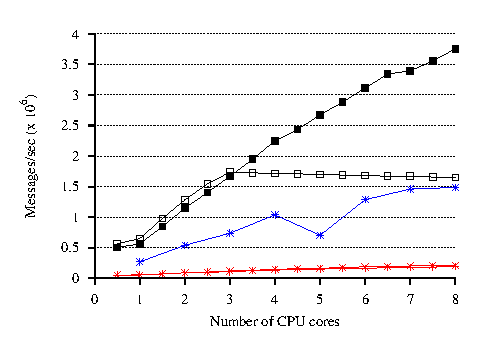
\includegraphics{figs/short-mcore-v2.eps}}
 \hspace{.01in}
 \subfloat[$n$ roundtrips per connection. (s=64B)]{
  \label{fig:short10:roundtrips}
  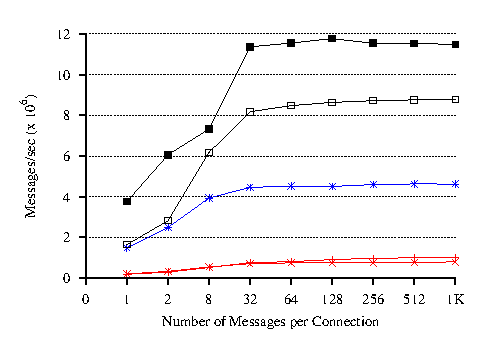
\includegraphics{figs/short-roundtrips-v2.eps}}
  \hspace{.01in}
 \subfloat[Different message sizes $s$ (n=1)]{
  \label{fig:short10:size}
  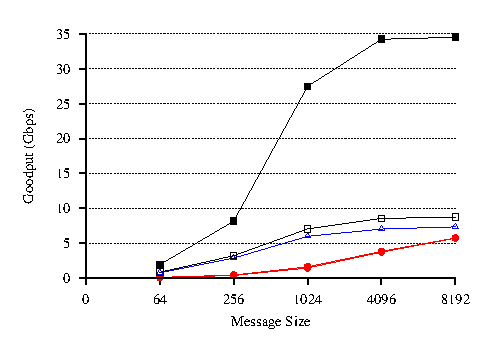
\includegraphics{figs/short-size-v2.eps}}
 \centering

  \vspace{-7.8in}
  \subfloat{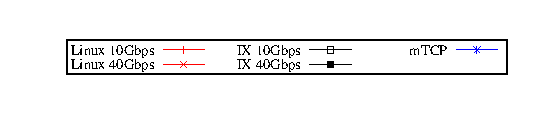
\includegraphics{figs/short-key-v2.eps}}
 \vspace{7in}


\caption{Multi-core scalability and high connection churn for 10GbE and 4x10GbE setups. \adam{In (a), half steps indicate hyperthreads.}}
 \label{fig:shortboth}

\end{figure}
